\documentclass{article}
\usepackage{listings}
\usepackage{hyperref}
\usepackage{graphicx}

\author{Tobias Dorra, Hendrik Schick}
\title{Project for Deep learning in medical imaging: Segmentation - MIC \\ \begin{large} 
Task 4: Implementation III
\end{large}}

\begin{document}
	
	\maketitle

	\section{Task}

		The task was to continue working on the Implementation.

	\section{Implementation}

		We fixed the last few remaining minor bugs. This allowed us, to run the final training for the liver dataset. We trained it for $25$ epochs, with the network architecture that is shown in figure~\ref{fig:model}. The training process took about $16$ hours.

		\begin{figure}[htbp]
			\centering
			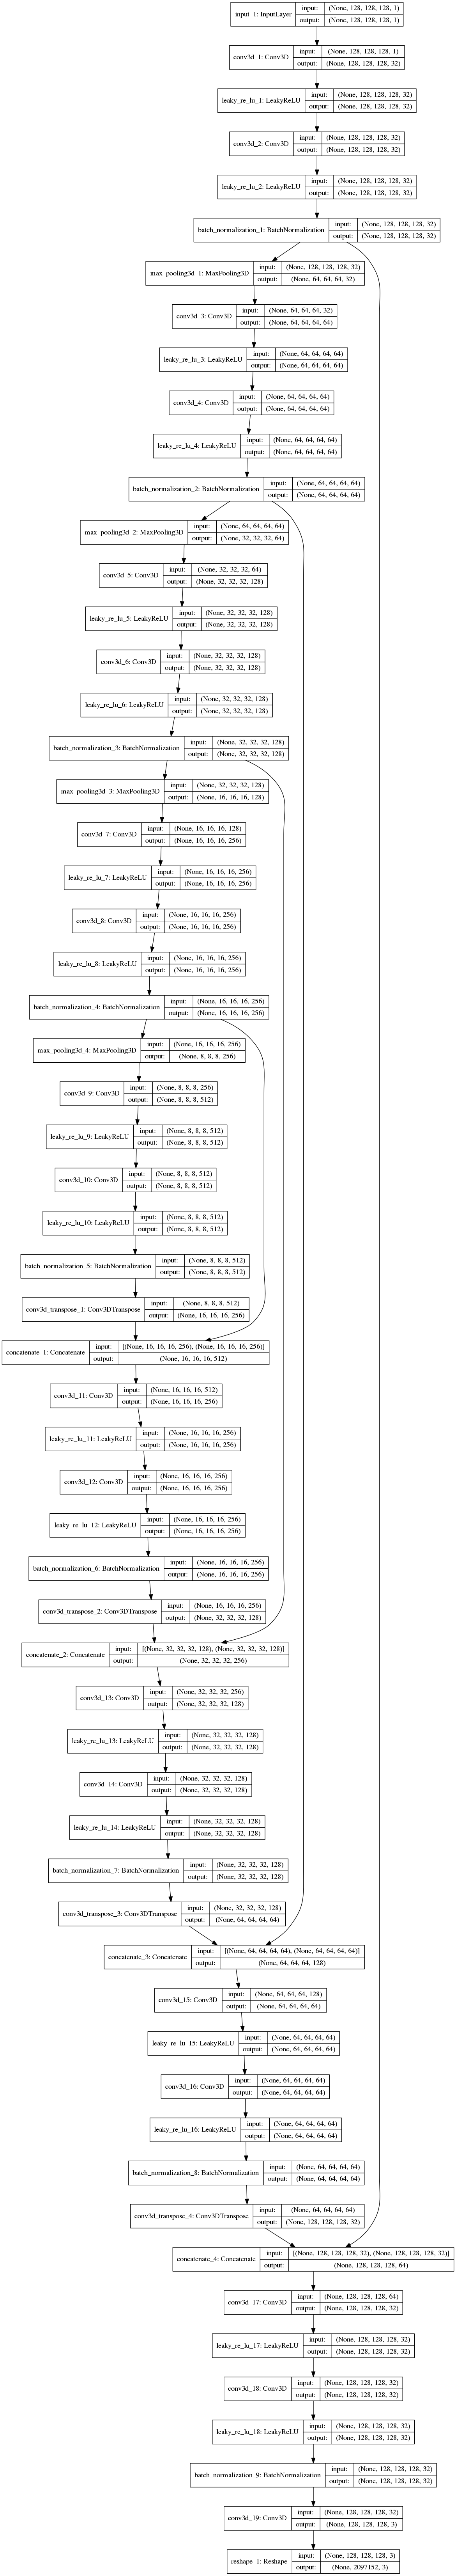
\includegraphics[height=\textheight]{model.png}
			\caption{Model architecture for the liver dataset.}
			(You should be able to zoom in to the pdf to see all the details - the image resolution is high enough.)
			\label{fig:model}
		\end{figure}

		If you look closely at the model architecture, you will see, that it changed a bit since the last time we showed it:

		\begin{itemize}
			\item The numbers of image channels has been decreased by factor 2. This is one differennce between nnUNet and our model, however it was neccessary in order to make the model work with the available GPU memory.
			\item There are additional BatchNormalization layers. The nnUNet paper mentions that they are using instance normalization. Since we have a batch size of 1, the batch normalization should be equivalent to instance normalization.
		\end{itemize}

		During training, we logged both the training- and test- loss. From that, we created figure~\ref{fig:lossdev}, that shows, how the losses develop over time during the training.

		\begin{figure}[htbp]
			\centering
			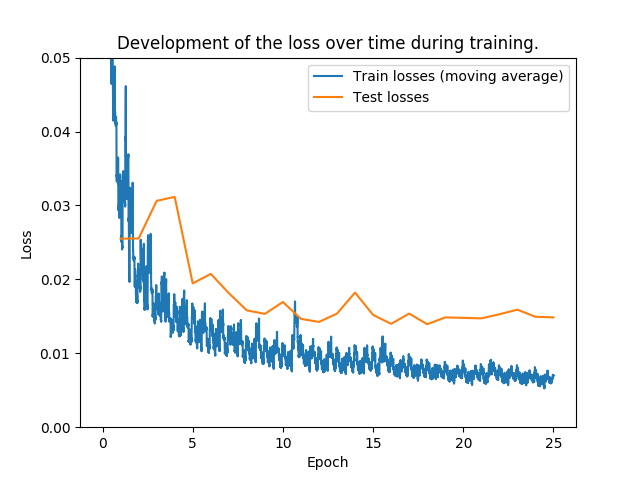
\includegraphics[width=.5\textwidth]{loss_over_time.png}
			\caption{Development of the loss during training}
			\label{fig:lossdev}
		\end{figure}

		In the figure, you can see, that the test loss does not really improve any more after epoch $16$. From that point on, the improvements of the training loss are probably just because of overfitting. So we could have stopped the training a bit earlier than we actually did.

		We evaluated the model performance on the ten unseen test images by calculating for each class the intersection over union between the real area that the class takes and the predicted one. The average values for the IOU are as follows:

		\begin{description}
			\item[Class 0] (outside): 0.98847
			\item[Class 1] (liver): 0.76387
			\item[Class 2] (cancer): 0.44024
		\end{description}

		The IOU for the cancer is the lowest, however, the areas of cancer are usually also quite small, so it is easy to miss a big percentage by being just a few pixels of.

		In order to be able to visually judge the quality of the model, we predicted the segmentation for the unseen images and stored them as images, next to corresponding images from the ground trueth. An example can be seen in figures~\ref{fig:pred} (predicted classes) and~\ref{fig:real} (ground truth). The corresponding input image is shown in figure~\ref{fig:inp}.

		\begin{figure}[htbp]
		 	\centering
		 	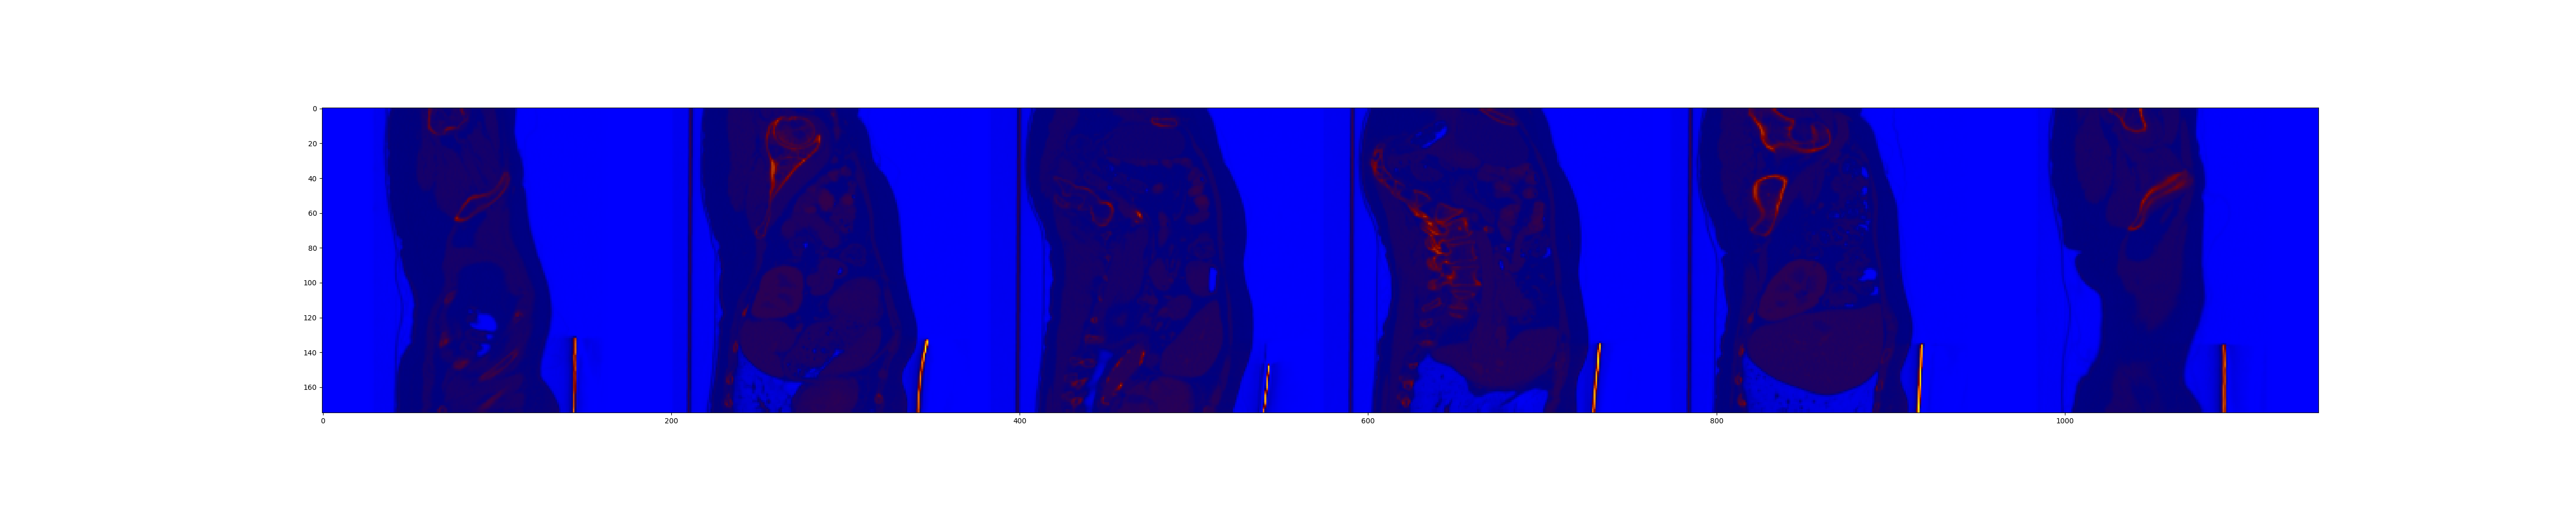
\includegraphics[width=\textwidth]{input.png}
		 	\caption{Input}
		 	\label{fig:inp}
		 \end{figure} 

		\begin{figure}[htbp]
		 	\centering
		 	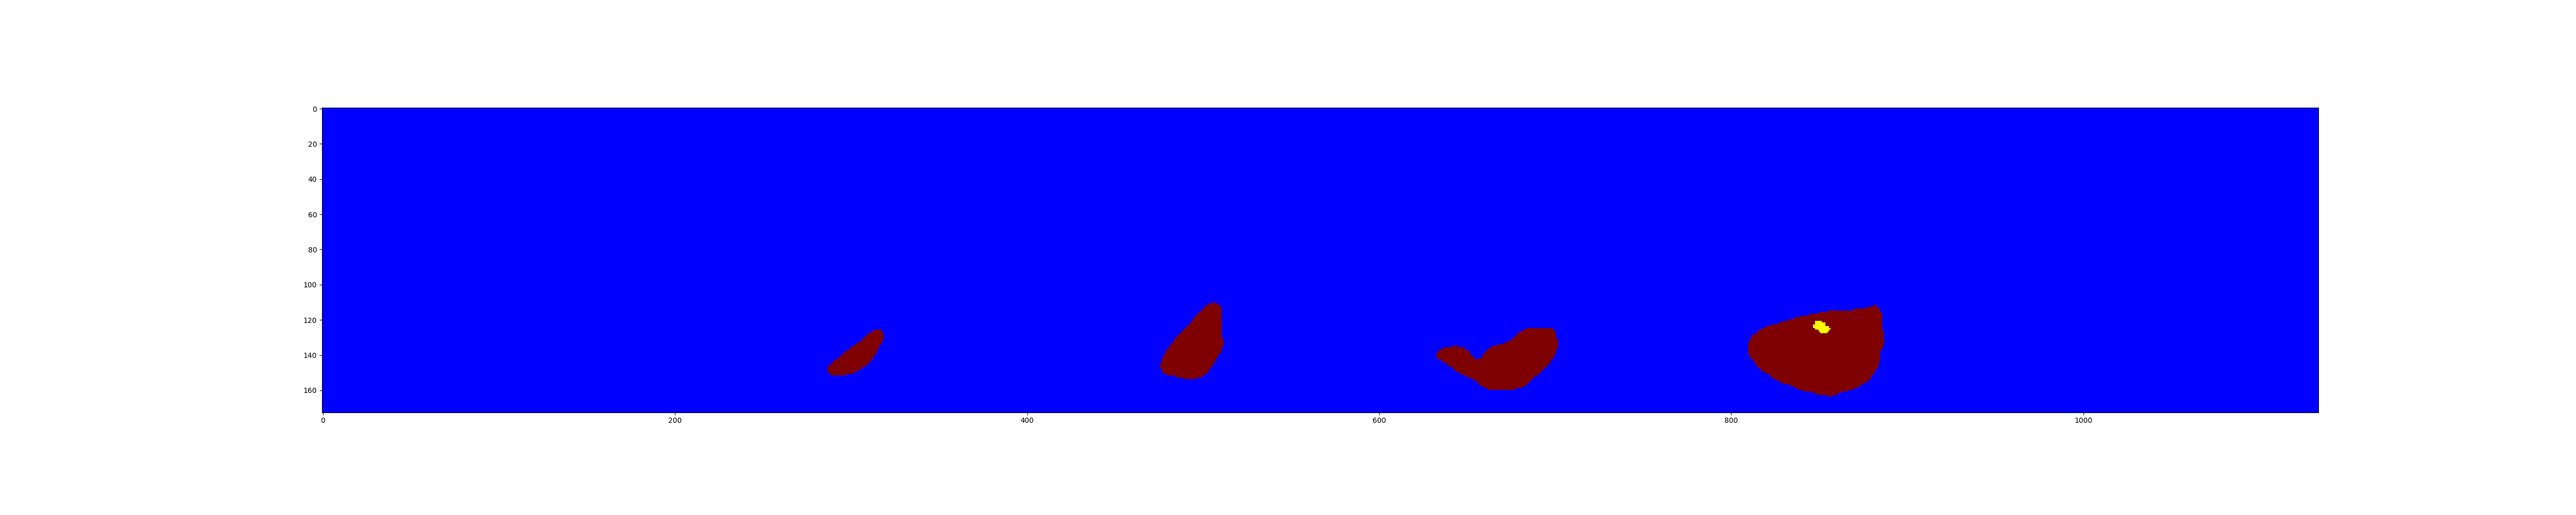
\includegraphics[width=\textwidth]{target.png}
		 	\caption{Real class labels}
		 	\label{fig:real}
		 \end{figure} 

		\begin{figure}[htbp]
		 	\centering
		 	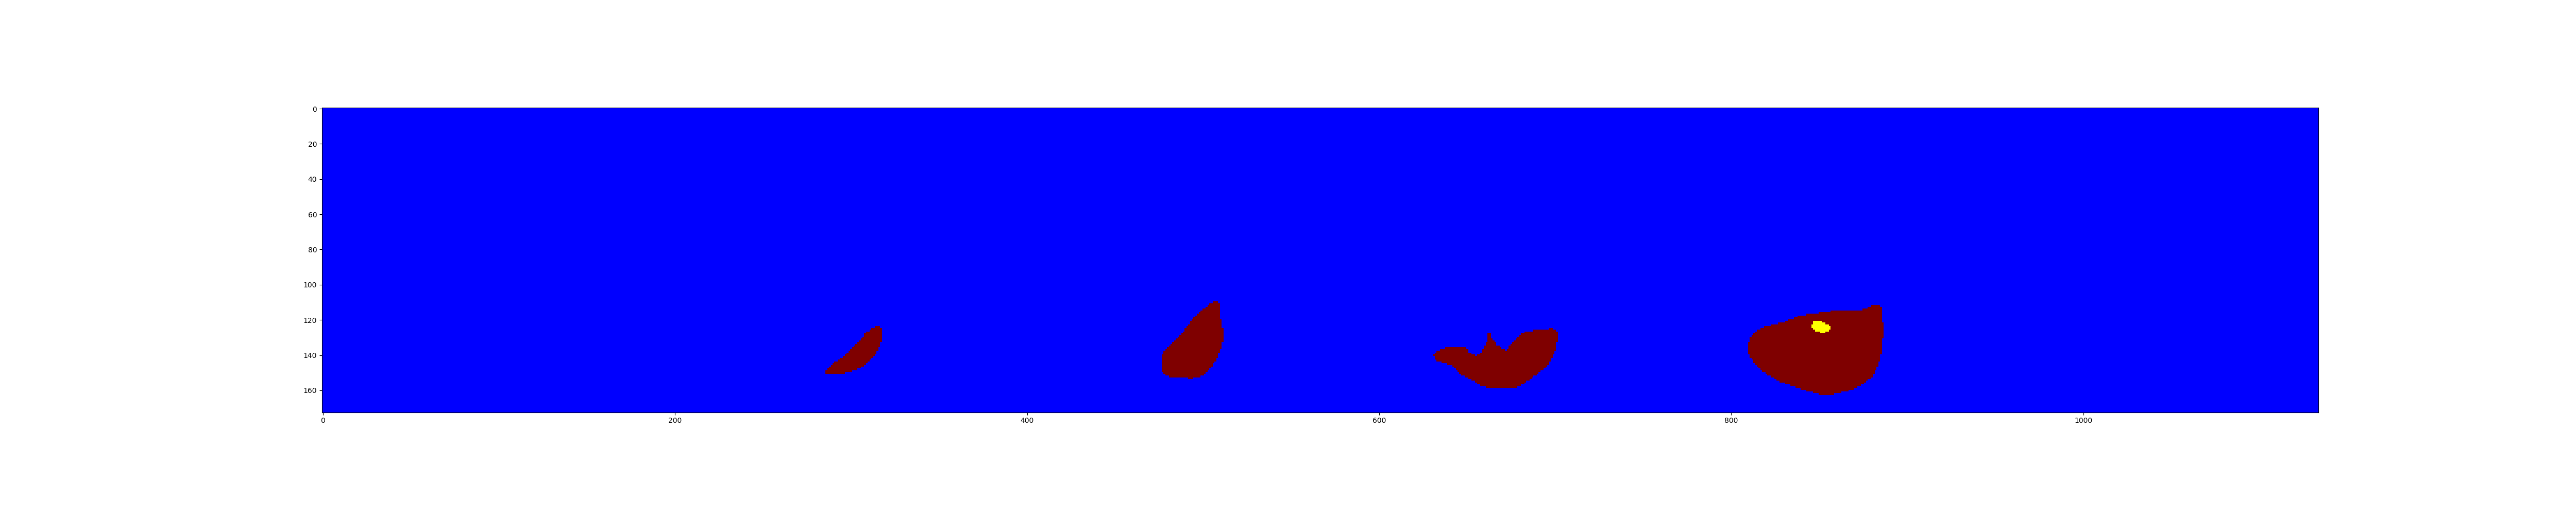
\includegraphics[width=\textwidth]{predicted.png}
		 	\caption{Predicted labels}
		 	\label{fig:pred}
		 \end{figure} 


	\section{Problems and future tasks}

		We still need to do the same evaluation procedure for the prostate dataset, but we can reuse our existing code for that, so it should be done pretty quickly and easily.

\end{document}
